\documentclass[11pt,a4paper]{article}

\usepackage[T1]{fontenc}
\usepackage[utf8]{inputenc}
\usepackage[frenchb]{babel}

\usepackage{fancyhdr} % headers
\usepackage[usenames,dvipsnames]{color} % colors
\usepackage{graphicx} % images
\usepackage{listings} % source code
\usepackage{titling} % meta-infos
\usepackage{courier} % courier font
\usepackage{fullpage} % full page layout
\usepackage{titlesec} % title customization
\usepackage{parskip} % paragraphs spacing
\usepackage{amsmath}
\usepackage{tikz}
\usepackage{siunitx}
%\usepackage{showframe} % layout debug

\usepackage{float}
\restylefloat{figure}

\topmargin -10mm
\headsep 5mm
\headheight 10mm

\linespread{1.1}
\renewcommand{\arraystretch}{1.3}

\setlength\parindent{0pt}
\setlength{\unitlength}{1cm}
\setlength{\droptitle}{-1.6cm}

\pagestyle{fancy}
\fancyhf{}
\cfoot{\thepage}

\def \doccourse { TIB1-B }
\def \doctitle {Rapport : Adressage IP}
\author{Bastien Clément \and Christophe Peretti}

\renewcommand{\thesection}{Objectif \arabic{section} :}
\renewcommand{\thesubsection}{\arabic{section}.\arabic{subsection}}

\rhead{\theauthor \\ \today}
\lhead{\doccourse \\ \doctitle }
\title{{\normalsize \doccourse} \\ \doctitle }

\begin{document}

\maketitle
\vspace{1em}

\section{Structure des adresses IP}

L'objectif de cette partie est d'apprendre la structure des adresses IP et de savoir calculer les adresses d'un réseau IP. Il est atteint si nous savons calculer, pour adresse IP en notation CIDR, le préfixe du réseau et la plage d'adresse de ce réseau.

\subsection{Tableau}

\begin{tabular}{|l|l|l|l|l|}
	\hline	
	\textbf{Propriétaire} & \textbf{Réseau} & \textbf{Première adr.} & \textbf{Dernière adr.} & \textbf{Nombre d'adr.} \\
	\hline
	EINEV2 & 193.134.216.0/21 & 192.134.216.0 & 192.134.223.255 & 2048 \\
	KSSG & 193.134.32.0/22 & 193.134.32.0 & 193.134.35.255 & 1024 \\
	UBS & 193.134.104.0/21 & 193.134.104.0 & 193.134.111.255 & 2048 \\
	SWISSRE & 193.134.160.0/20 & 193.134.160.0 & 193.134.178.255 & 4096 \\
	SOLO-NET & 193.134.64.0/19 & 193.134.64.0 & 193.134.95.255 & 8192 \\
	\hline
\end{tabular}

\subsection{À partir de $a.b.c.d/x$ calculer le préfixe réseau}

Le préfixe réseau est composé des $x$ premiers bits de l'adresse. L'algorithme basique consiste à convertir l'adresse complète en binaire, de construire un masque de $x$ bits puis d'appliquer l'opération ET entre les deux. Il est possible de se simplifier la tâche en identifiant quel octet est partagé entre le préfixe et l'adresse.

Pour cela, nous effectuons la division euclidienne de $x$ par 8. Le \textit{quotient} est le nombre d'octets à conserver tel quel dans le préfixe. Le \textit{reste} est le nombre de bits de l'octet suivant faisant partie du préfixe réseau. L'opération de masquage peut alors être effectuée sur 8 bits au lieu de 32. Les octets suivants sont finalement changés en 0. 
Dans le cas où $x$ est un multiple de 8, aucune opération de masquage est nécessaire et le problème est trivial.

\subsection{À partir de $a.b.c.d/x$ calculer la plage d'adresses de ce réseau}

Si $x$ bits sont utilisés pour le préfixe réseau, il en reste $(32-x)$ pour adresser les machines de ce réseau. Par conséquent, il y a $2^{(32-x)}$ adresses possibles.

\subsection{Exemple à partir l'adresse $193.34.232.12/18$}

\subsubsection*{Préfixe réseau}

$18 = 2 \times 8 + 2$

Les deux premiers octets peuvent donc être conservés et seul le troisième octet a besoin d'être converti en binaire pour appliquer l'opération de masquage:

\begin{tabular}{rclcl}
	$232_{10}$ & $=$ & $1110 1000_2$ \\
	& \& & $1100 0000$ \\
	\hline
	& & $1100 0000_2$ & $=$ & $192_{10}$
\end{tabular}

Le réseau est donc 193.24.192.0.

\subsubsection*{Plage d'adresse}

$2^{32-18} = 2^{14} = 16384$

\section{Remise directe et remise indirecte}

L'objectif de cette partie est de comprendre la différence entre remise directe et remise indirecte de paquets IP. L'objectif est atteint si nous savons expliquer comment un paquet est transmis à un destinataire dans le même réseau ou à un destinataire dans un autre réseau.

\subsection{Différences}

En théorie, toutes les machines d'un réseau Ethernet partagent un médium de transmission commun sur lequel une seule d'entre-elles peut transmettre des informations à un instant donné. En divisant un réseau de taille importante en sous-réseaux, il est possible de créer plusieurs domaines de collision et ainsi permettre aux machines de communiquer simultanément dans leurs sous-réseaux respectifs.

Pour permettre à une machine d'un sous-réseau de communiquer avec une machine d'un autre sous-réseau, il est alors nécessaire de disposer d'un \textit{routeur}, connecté simultanément aux deux sous-réseaux et faisant office de pont. Une machine ne peut alors communiquer directement qu'avec les machines du même sous-réseau et doit utiliser ce routeur pour communiquer indirectement avec une machine d'un autre sous-réseau.

Dans le cas d'une remise directe, le protocole ARP est utilisé pour obtenir l'adresse MAC de la machine destinataire puis le paquet IP est transmis directement à cette machine.

Dans le cas d'une remise indirecte, le protocole ARP est utilisé pour obtenir l'adresse MAC du routeur. Le paquet IP est toujours adressé à la machine destinataire mais la trame Ethernet l'encapsulant est adressée au routeur. À la réception d'un paquet IP qui ne lui est pas directement adressé, il se chargera de le relayer pour atteindre la bonne destination.

\subsection{Exemple de remise directe}

\begin{center}
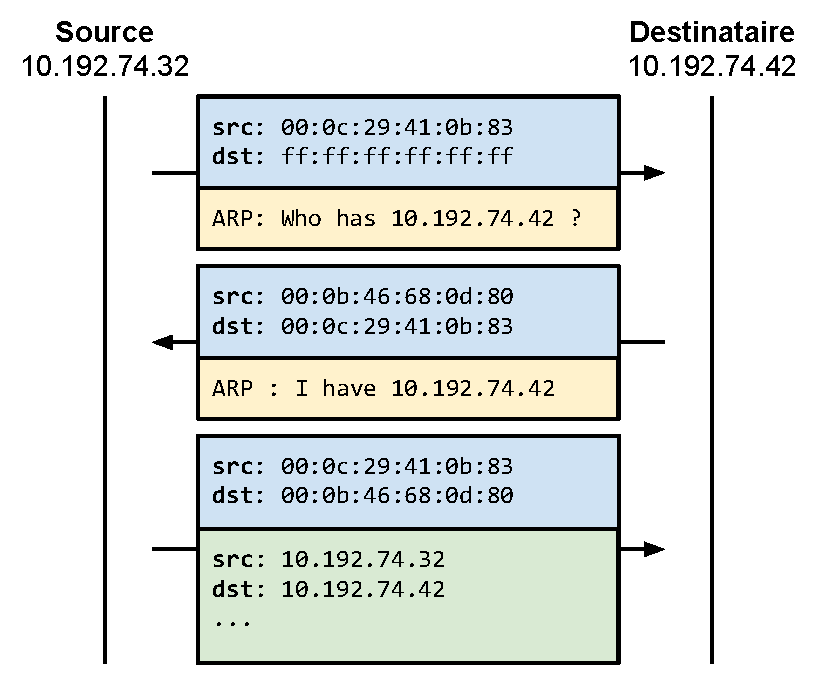
\includegraphics[width=8.5cm]{img_direct}
\end{center}

Ceci est le processus de remise habituel que nous avons observé dans les laboratoires précédents.

\subsection{Exemple de remise indirecte}

\begin{center}
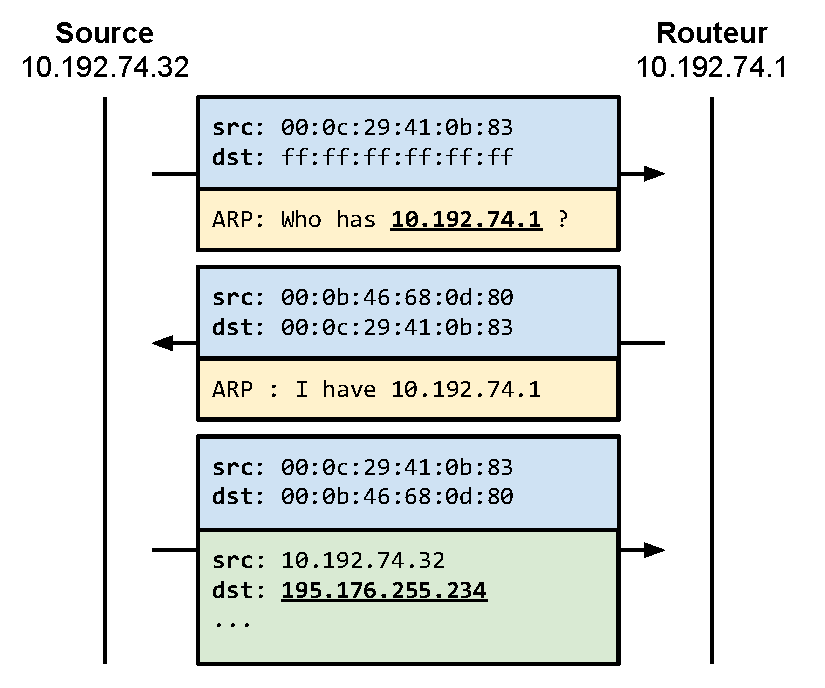
\includegraphics[width=8.5cm]{img_indirect}
\end{center}

On observe clairement la différence entre l'adresse MAC de destination de la trame (correspondant au routeur) et l'adresse IP qui est celle de la machine de destination finale.

Le routeur répète alors le processus pour effectuer une remise directe ou indirecte selon que la machine soit ou non située dans un réseau auquel il est connecté.

\section{Auto-évaluation}

Nous considérons avoir atteint les objectifs de ce laboratoire.

\end{document}